\documentclass[11pt]{article}
\usepackage{graphicx}
\usepackage{hyperref}
\usepackage{longtable}
\usepackage[margin=.7in]{geometry}


\begin{document}

\title{CSE564 Visualization}
\author{Yinlong Su, \#110461173}
\maketitle

\section*{Raw Data Report}

\setcounter{section}{-1}
\section{Version History}

First built on April 10, 2016.

\section{CSV Report}

There are 65,503 rows and 159 columns in raw data.

\section{Column Report}

Many columns are incomplete. Some missing data is unrecoverable, while some can be filled as default value. For example, column ``lignoceric\_acid\_100g" are empty so intuitively we know that the food has no lignoceric acid.
\par
Here we roughly divide the data type into 5 types: Numeric, Text, Time, URL and Unknown. See table \ref{tab:columnReportTable}.
\par

\begin{center}
\begin{longtable}{|l|c|r|}
\caption[Column Report Table]{Column Report Table} \label{tab:columnReportTable} \\
\hline
\multicolumn{1}{|c|}{\textbf{Column Name}} & \multicolumn{1}{c|}{\textbf{Type}} & \multicolumn{1}{c|} {\textbf{Empty/Invalid}} \\
\hline
\endfirsthead

\multicolumn{3}{c}%
{{\bfseries \tablename\ \thetable{} -- continued from previous page}} \\
\hline
\multicolumn{1}{|c|}{\textbf{Column Name}} & \multicolumn{1}{c|}{\textbf{Type}} & \multicolumn{1}{c|} {\textbf{Empty/Invalid}} \\
\hline
\endhead

\hline \multicolumn{3}{|r|}{{Continued on next page}} \\
\hline
\endfoot

\hline
\hline
\endlastfoot

code& numericType& 17 (0.03\%)\\
url& urlType& 17 (0.03\%)\\
creator& textType& 68 (0.1\%)\\
created\_t& timeType& 3 (0.0\%)\\
created\_datetime& timeType& 7 (0.01\%)\\
last\_modified\_t& timeType& 0 (0.0\%)\\
last\_modified\_datetime& timeType& 0 (0.0\%)\\
product\_name& textType& 5230 (7.98\%)\\
generic\_name& textType& 31290 (47.77\%)\\
quantity& textType& 9218 (14.07\%)\\
packaging& textType& 15425 (23.55\%)\\
packaging\_tags& textType& 15425 (23.55\%)\\
brands& textType& 9303 (14.2\%)\\
brands\_tags& textType& 9304 (14.2\%)\\
categories& textType& 15608 (23.83\%)\\
categories\_tags& textType& 15623 (23.85\%)\\
categories\_en& textType& 15607 (23.83\%)\\
origins& textType& 50138 (76.54\%)\\
origins\_tags& textType& 50175 (76.6\%)\\
manufacturing\_places& textType& 44435 (67.84\%)\\
manufacturing\_places\_tags& textType& 44441 (67.85\%)\\
labels& textType& 40756 (62.22\%)\\
labels\_tags& textType& 40709 (62.15\%)\\
labels\_en& textType& 40693 (62.12\%)\\
emb\_codes& textType& 46138 (70.44\%)\\
emb\_codes\_tags& textType& 46141 (70.44\%)\\
first\_packaging\_code\_geo& textType& 53278 (81.34\%)\\
cities& textType& 65487 (99.98\%)\\
cities\_tags& textType& 52241 (79.75\%)\\
purchase\_places& textType& 28271 (43.16\%)\\
stores& textType& 33419 (51.02\%)\\
countries& textType& 211 (0.32\%)\\
countries\_tags& textType& 211 (0.32\%)\\
countries\_en& textType& 211 (0.32\%)\\
ingredients\_text& textType& 21822 (33.31\%)\\
allergens& textType& 51966 (79.33\%)\\
allergens\_en& textType& 65486 (99.97\%)\\
traces& textType& 50631 (77.3\%)\\
traces\_tags& textType& 50649 (77.32\%)\\
traces\_en& textType& 50633 (77.3\%)\\
serving\_size& textType& 44329 (67.67\%)\\
no\_nutriments& unknownType& 65503 (100.0\%)\\
additives\_n& numericType& 21839 (33.34\%)\\
additives& textType& 21857 (33.37\%)\\
additives\_tags& textType& 41838 (63.87\%)\\
additives\_en& textType& 41838 (63.87\%)\\
ingredients\_from\_palm\_oil\_n& numericType& 21839 (33.34\%)\\
ingredients\_from\_palm\_oil& textType& 65503 (100.0\%)\\
ingredients\_from\_palm\_oil\_tags& textType& 63122 (96.37\%)\\
ingredients\_that\_may\_be\_from\_palm\_oil\_n& numericType& 21839 (33.34\%)\\
ingredients\_that\_may\_be\_from\_palm\_oil& textType& 65503 (100.0\%)\\
ingredients\_that\_may\_be\_from\_palm\_oil\_tags& textType& 60981 (93.1\%)\\
nutrition\_grade\_uk& textType& 65503 (100.0\%)\\
nutrition\_grade\_fr& textType& 34209 (52.23\%)\\
pnns\_groups\_1& textType& 12997 (19.84\%)\\
pnns\_groups\_2& textType& 11087 (16.93\%)\\
states& textType& 88 (0.13\%)\\
states\_tags& textType& 88 (0.13\%)\\
states\_en& textType& 88 (0.13\%)\\
main\_category& textType& 15640 (23.88\%)\\
main\_category\_en& textType& 15640 (23.88\%)\\
image\_url& urlType& 4304 (6.57\%)\\
image\_small\_url& urlType& 4304 (6.57\%)\\
energy\_100g& numericType& 29129 (44.47\%)\\
energy\_from\_fat\_100g& numericType& 64770 (98.88\%)\\
fat\_100g& numericType& 29141 (44.49\%)\\
saturated\_fat\_100g& numericType& 33074 (50.49\%)\\
butyric\_acid\_100g& numericType& 65503 (100.0\%)\\
caproic\_acid\_100g& numericType& 65503 (100.0\%)\\
caprylic\_acid\_100g& numericType& 65502 (100.0\%)\\
capric\_acid\_100g& numericType& 65502 (100.0\%)\\
lauric\_acid\_100g& numericType& 65500 (100.0\%)\\
myristic\_acid\_100g& numericType& 65502 (100.0\%)\\
palmitic\_acid\_100g& numericType& 65502 (100.0\%)\\
stearic\_acid\_100g& numericType& 65502 (100.0\%)\\
arachidic\_acid\_100g& numericType& 65486 (99.97\%)\\
behenic\_acid\_100g& numericType& 65487 (99.98\%)\\
lignoceric\_acid\_100g& numericType& 65503 (100.0\%)\\
cerotic\_acid\_100g& numericType& 65503 (100.0\%)\\
montanic\_acid\_100g& numericType& 65503 (100.0\%)\\
melissic\_acid\_100g& numericType& 65503 (100.0\%)\\
monounsaturated\_fat\_100g& numericType& 63946 (97.62\%)\\
polyunsaturated\_fat\_100g& numericType& 63933 (97.6\%)\\
omega\_3\_fat\_100g& numericType& 64976 (99.2\%)\\
alpha\_linolenic\_acid\_100g& numericType& 65374 (99.8\%)\\
eicosapentaenoic\_acid\_100g& numericType& 65470 (99.95\%)\\
docosahexaenoic\_acid\_100g& numericType& 65446 (99.91\%)\\
omega\_6\_fat\_100g& numericType& 65366 (99.79\%)\\
linoleic\_acid\_100g& numericType& 65406 (99.85\%)\\
arachidonic\_acid\_100g& numericType& 65498 (99.99\%)\\
gamma\_linolenic\_acid\_100g& numericType& 65486 (99.97\%)\\
dihomo\_gamma\_linolenic\_acid\_100g& numericType& 65487 (99.98\%)\\
omega\_9\_fat\_100g& numericType& 65487 (99.98\%)\\
oleic\_acid\_100g& numericType& 65496 (99.99\%)\\
elaidic\_acid\_100g& numericType& 65503 (100.0\%)\\
gondoic\_acid\_100g& numericType& 65495 (99.99\%)\\
mead\_acid\_100g& numericType& 65503 (100.0\%)\\
erucic\_acid\_100g& numericType& 65503 (100.0\%)\\
nervonic\_acid\_100g& numericType& 65503 (100.0\%)\\
trans\_fat\_100g& numericType& 64275 (98.13\%)\\
cholesterol\_100g& numericType& 64112 (97.88\%)\\
carbohydrates\_100g& numericType& 29438 (44.94\%)\\
sugars\_100g& numericType& 32864 (50.17\%)\\
sucrose\_100g& numericType& 65495 (99.99\%)\\
glucose\_100g& numericType& 65498 (99.99\%)\\
fructose\_100g& numericType& 65483 (99.97\%)\\
lactose\_100g& numericType& 65362 (99.78\%)\\
maltose\_100g& numericType& 65501 (100.0\%)\\
maltodextrins\_100g& numericType& 65496 (99.99\%)\\
starch\_100g& numericType& 65287 (99.67\%)\\
polyols\_100g& numericType& 65253 (99.62\%)\\
fiber\_100g& numericType& 42957 (65.58\%)\\
proteins\_100g& numericType& 29573 (45.15\%)\\
casein\_100g& numericType& 65488 (99.98\%)\\
serum\_proteins\_100g& numericType& 65495 (99.99\%)\\
nucleotides\_100g& numericType& 65500 (100.0\%)\\
salt\_100g& numericType& 32595 (49.76\%)\\
sodium\_100g& numericType& 32605 (49.78\%)\\
alcohol\_100g& numericType& 63084 (96.31\%)\\
vitamin\_a\_100g& numericType& 64142 (97.92\%)\\
beta\_carotene\_100g& numericType& 65494 (99.99\%)\\
vitamin\_d\_100g& numericType& 64921 (99.11\%)\\
vitamin\_e\_100g& numericType& 64746 (98.84\%)\\
vitamin\_k\_100g& numericType& 65444 (99.91\%)\\
vitamin\_c\_100g& numericType& 63595 (97.09\%)\\
vitamin\_b1\_100g& numericType& 64632 (98.67\%)\\
vitamin\_b2\_100g& numericType& 64782 (98.9\%)\\
vitamin\_pp\_100g& numericType& 64772 (98.88\%)\\
vitamin\_b6\_100g& numericType& 64800 (98.93\%)\\
vitamin\_b9\_100g& numericType& 64766 (98.87\%)\\
vitamin\_b12\_100g& numericType& 64912 (99.1\%)\\
biotin\_100g& numericType& 65310 (99.71\%)\\
pantothenic\_acid\_100g& numericType& 65096 (99.38\%)\\
silica\_100g& numericType& 65475 (99.96\%)\\
bicarbonate\_100g& numericType& 65441 (99.91\%)\\
potassium\_100g& numericType& 65006 (99.24\%)\\
chloride\_100g& numericType& 65397 (99.84\%)\\
calcium\_100g& numericType& 62554 (95.5\%)\\
phosphorus\_100g& numericType& 64913 (99.1\%)\\
iron\_100g& numericType& 63650 (97.17\%)\\
magnesium\_100g& numericType& 64706 (98.78\%)\\
zinc\_100g& numericType& 65258 (99.63\%)\\
copper\_100g& numericType& 65407 (99.85\%)\\
manganese\_100g& numericType& 65418 (99.87\%)\\
fluoride\_100g& numericType& 65448 (99.92\%)\\
selenium\_100g& numericType& 65429 (99.89\%)\\
chromium\_100g& numericType& 65488 (99.98\%)\\
molybdenum\_100g& numericType& 65498 (99.99\%)\\
iodine\_100g& numericType& 65388 (99.82\%)\\
caffeine\_100g& numericType& 65467 (99.95\%)\\
taurine\_100g& numericType& 65487 (99.98\%)\\
ph\_100g& numericType& 65468 (99.95\%)\\
fruits\_vegetables\_nuts\_100g& numericType& 64474 (98.43\%)\\
collagen\_meat\_protein\_ratio\_100g& numericType& 65394 (99.83\%)\\
cocoa\_100g& numericType& 65071 (99.34\%)\\
chlorophyl\_100g& numericType& 65503 (100.0\%)\\
carbon\_footprint\_100g& numericType& 65323 (99.73\%)\\
nutrition\_score\_fr\_100g& numericType& 34209 (52.23\%)\\
nutrition\_score\_uk\_100g& numericType& 34209 (52.23\%)\\


\hline

\end{longtable}
\end{center}

Figure \ref{fig:columnReportFigure} shows the level of integrities of the columns.

\begin{figure}[!htp]
\centering
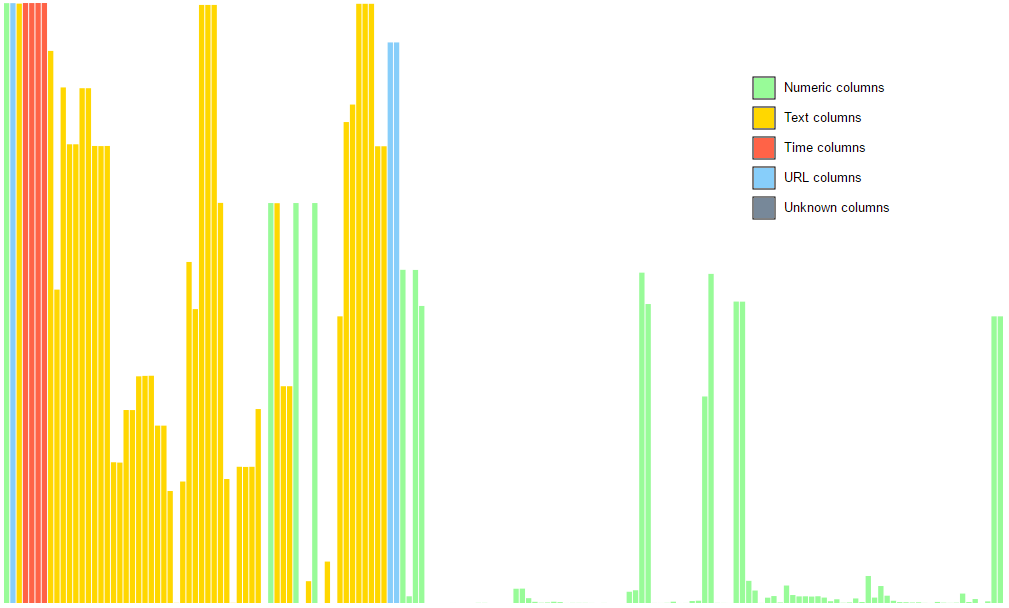
\includegraphics[width=\textwidth]{../vis/integrities.of.raw.columns.png}
\caption{Integrities of Raw Columns}
\label{fig:columnReportFigure}
\end{figure}

\section{Numeric Columns Report}

Table \ref{tab:numericColumnReportTable} shows the report of numeric columns. I ommited the average values, see ``raw.analysis.txt" if you need them.

\begin{center}
\begin{longtable}{|l|r|r|r|}
\caption[Numeric Column Report Table]{Numeric Column Report Table} \label{tab:numericColumnReportTable} \\
\hline
\multicolumn{1}{|c|}{\textbf{Column Name}} & \multicolumn{1}{c|}{\textbf{Min}} & \multicolumn{1}{c|}{\textbf{Max}} & \multicolumn{1}{c|} {\textbf{Empty/Invalid}} \\
\hline
\endfirsthead

\multicolumn{4}{c}%
{{\bfseries \tablename\ \thetable{} -- continued from previous page}} \\
\hline
\multicolumn{1}{|c|}{\textbf{Column Name}} & \multicolumn{1}{c|}{\textbf{Min}} & \multicolumn{1}{c|}{\textbf{Max}} & \multicolumn{1}{c|} {\textbf{Empty/Invalid}} \\
\hline
\endhead

\hline \multicolumn{4}{|r|}{{Continued on next page}} \\
\hline
\endfoot

\hline
\hline
\endlastfoot

additives\_n& 0.0& 26.0& 21839 (33.34\%)\\
ingredients\_from\_palm\_oil\_n& 0.0& 2.0& 21839 (33.34\%)\\
ingredients\_that\_may\_be\_from\_palm\_oil\_n& 0.0& 6.0& 21839 (33.34\%)\\
energy\_100g& 0.0& 4134.0& 29129 (44.47\%)\\
energy\_from\_fat\_100g& 0.0& 3740.0& 64770 (98.88\%)\\
fat\_100g& 0.0& 101.0& 29141 (44.49\%)\\
saturated\_fat\_100g& 0.0& 100.0& 33074 (50.49\%)\\
butyric\_acid\_100g& nan& nan& 65503 (100.0\%)\\
caproic\_acid\_100g& nan& nan& 65503 (100.0\%)\\
caprylic\_acid\_100g& 7.4& 7.4& 65502 (100.0\%)\\
capric\_acid\_100g& 6.2& 6.2& 65502 (100.0\%)\\
lauric\_acid\_100g& 0.04473& 49.3& 65500 (100.0\%)\\
myristic\_acid\_100g& 18.9& 18.9& 65502 (100.0\%)\\
palmitic\_acid\_100g& 8.1& 8.1& 65502 (100.0\%)\\
stearic\_acid\_100g& 3.0& 3.0& 65502 (100.0\%)\\
arachidic\_acid\_100g& 0.064& 15.4& 65486 (99.97\%)\\
behenic\_acid\_100g& 5.5& 14.6& 65487 (99.98\%)\\
lignoceric\_acid\_100g& nan& nan& 65503 (100.0\%)\\
cerotic\_acid\_100g& nan& nan& 65503 (100.0\%)\\
montanic\_acid\_100g& nan& nan& 65503 (100.0\%)\\
melissic\_acid\_100g& nan& nan& 65503 (100.0\%)\\
monounsaturated\_fat\_100g& 0.0& 80.0& 63946 (97.62\%)\\
polyunsaturated\_fat\_100g& 0.0& 74.0& 63933 (97.6\%)\\
omega\_3\_fat\_100g& 0.00015& 38.2& 64976 (99.2\%)\\
alpha\_linolenic\_acid\_100g& 0.0& 47.0& 65374 (99.8\%)\\
eicosapentaenoic\_acid\_100g& 0.048& 85.0& 65470 (99.95\%)\\
docosahexaenoic\_acid\_100g& 0.044& 12.0& 65446 (99.91\%)\\
omega\_6\_fat\_100g& 0.05& 71.0& 65366 (99.79\%)\\
linoleic\_acid\_100g& 0.09& 25.0& 65406 (99.85\%)\\
arachidonic\_acid\_100g& 0.007& 0.09& 65498 (99.99\%)\\
gamma\_linolenic\_acid\_100g& 0.095& 0.2032& 65486 (99.97\%)\\
dihomo\_gamma\_linolenic\_acid\_100g& 0.05& 0.08& 65487 (99.98\%)\\
omega\_9\_fat\_100g& 1.0& 75.0& 65487 (99.98\%)\\
oleic\_acid\_100g& 1.08& 70.0& 65496 (99.99\%)\\
elaidic\_acid\_100g& nan& nan& 65503 (100.0\%)\\
gondoic\_acid\_100g& 1e-06& 1.25e-06& 65495 (99.99\%)\\
mead\_acid\_100g& nan& nan& 65503 (100.0\%)\\
erucic\_acid\_100g& nan& nan& 65503 (100.0\%)\\
nervonic\_acid\_100g& nan& nan& 65503 (100.0\%)\\
trans\_fat\_100g& 0.0& 30.3& 64275 (98.13\%)\\
cholesterol\_100g& 0.0& 0.432& 64112 (97.88\%)\\
carbohydrates\_100g& 0.0& 139.0& 29438 (44.94\%)\\
sugars\_100g& -0.5& 105.0& 32864 (50.17\%)\\
sucrose\_100g& 0.0& 8.4& 65495 (99.99\%)\\
glucose\_100g& 0.1& 2.0& 65498 (99.99\%)\\
fructose\_100g& 0.1& 101.0& 65483 (99.97\%)\\
lactose\_100g& 0.0& 58.5& 65362 (99.78\%)\\
maltose\_100g& 0.1& 22.0& 65501 (100.0\%)\\
maltodextrins\_100g& 1.8& 27.5& 65496 (99.99\%)\\
starch\_100g& 0.0& 87.8& 65287 (99.67\%)\\
polyols\_100g& 0.0& 100.0& 65253 (99.62\%)\\
fiber\_100g& 0.0& 94.8& 42957 (65.58\%)\\
proteins\_100g& 0.0& 86.0& 29573 (45.15\%)\\
casein\_100g& 0.92& 10.2& 65488 (99.98\%)\\
serum\_proteins\_100g& 0.3& 5.8& 65495 (99.99\%)\\
nucleotides\_100g& 0.018& 0.024& 65500 (100.0\%)\\
salt\_100g& 0.0& 254.0& 32595 (49.76\%)\\
sodium\_100g& 0.0& 100.0& 32605 (49.78\%)\\
alcohol\_100g& 0.0& 97.9& 63084 (96.31\%)\\
vitamin\_a\_100g& 0.0& 26.7& 64142 (97.92\%)\\
beta\_carotene\_100g& 0.000812& 0.26& 65494 (99.99\%)\\
vitamin\_d\_100g& 0.0& 7.5& 64921 (99.11\%)\\
vitamin\_e\_100g& 0.0& 15.1& 64746 (98.84\%)\\
vitamin\_k\_100g& 0.0& 0.0334& 65444 (99.91\%)\\
vitamin\_c\_100g& 0.0& 100.0& 63595 (97.09\%)\\
vitamin\_b1\_100g& 1e-05& 0.169& 64632 (98.67\%)\\
vitamin\_b2\_100g& 0.0& 30.0& 64782 (98.9\%)\\
vitamin\_pp\_100g& 2.4e-06& 15.9& 64772 (98.88\%)\\
vitamin\_b6\_100g& 0.0& 0.215& 64800 (98.93\%)\\
vitamin\_b9\_100g& 0.0& 4.0& 64766 (98.87\%)\\
vitamin\_b12\_100g& 0.0& 50.0& 64912 (99.1\%)\\
biotin\_100g& -2.0& 5.0& 65310 (99.71\%)\\
pantothenic\_acid\_100g& -2.0& 5.0& 65096 (99.38\%)\\
silica\_100g& 8.2e-06& 0.0362& 65475 (99.96\%)\\
bicarbonate\_100g& 6.3e-06& 1.1& 65441 (99.91\%)\\
potassium\_100g& 0.0& 34.6& 65006 (99.24\%)\\
chloride\_100g& 2e-06& 0.5& 65397 (99.84\%)\\
calcium\_100g& 0.0& 69.5& 62554 (95.5\%)\\
phosphorus\_100g& 0.0012& 84.9& 64913 (99.1\%)\\
iron\_100g& 0.0& 19.2& 63650 (97.17\%)\\
magnesium\_100g& 5e-07& 11.5& 64706 (98.78\%)\\
zinc\_100g& 0.0001& 4.0& 65258 (99.63\%)\\
copper\_100g& 1.67e-05& 0.35& 65407 (99.85\%)\\
manganese\_100g& 3e-06& 0.7& 65418 (99.87\%)\\
fluoride\_100g& 0.0& 0.56& 65448 (99.92\%)\\
selenium\_100g& 7e-07& 0.03& 65429 (99.89\%)\\
chromium\_100g& 7.06e-06& 0.0001& 65488 (99.98\%)\\
molybdenum\_100g& 7e-06& 4.5e-05& 65498 (99.99\%)\\
iodine\_100g& 3.6e-09& 0.0147& 65388 (99.82\%)\\
caffeine\_100g& 0.003& 32.0& 65467 (99.95\%)\\
taurine\_100g& 0.0018& 0.423& 65487 (99.98\%)\\
ph\_100g& 0.005& 7.9& 65468 (99.95\%)\\
fruits\_vegetables\_nuts\_100g& 1.4& 100.0& 64474 (98.43\%)\\
collagen\_meat\_protein\_ratio\_100g& 8.0& 25.0& 65394 (99.83\%)\\
cocoa\_100g& 6.3& 100.0& 65071 (99.34\%)\\
chlorophyl\_100g& nan& nan& 65503 (100.0\%)\\
carbon\_footprint\_100g& 0.0& 2842.0& 65323 (99.73\%)\\
nutrition\_score\_fr\_100g& -14.0& 35.0& 34209 (52.23\%)\\
nutrition\_score\_uk\_100g& -14.0& 33.0& 34209 (52.23\%)\\

\hline

\end{longtable}
\end{center}


\section{Text Group Columns Report}
Table \ref{tab:textGroupColumnReportTable} shows the number of different values on selected text columns. Some of the columns are actually multiset of text information. The number is too large to be reasonably group. Further processing is needed.

\begin{center}
\begin{longtable}{|l|r|r|}
\caption[Text Group Column Report Table]{Text Group Column Report Table} \label{tab:textGroupColumnReportTable} \\
\hline
\multicolumn{1}{|c|}{\textbf{Column Name}} & \multicolumn{1}{c|}{\textbf{Group \#}} & \multicolumn{1}{c|} {\textbf{Empty/Invalid}} \\
\hline
\endfirsthead

\multicolumn{3}{c}%
{{\bfseries \tablename\ \thetable{} -- continued from previous page}} \\
\hline
\multicolumn{1}{|c|}{\textbf{Column Name}} & \multicolumn{1}{c|}{\textbf{Group \#}} & \multicolumn{1}{c|} {\textbf{Empty/Invalid}} \\
\hline
\endhead

\hline \multicolumn{3}{|r|}{{Continued on next page}} \\
\hline
\endfoot

\hline
\hline
\endlastfoot

creator& 1905& 68 (0.1\%)\\
brands& 17172& 9303 (14.2\%)\\
brands\_tags& 14097& 9304 (14.2\%)\\
categories& 23878& 15608 (23.83\%)\\
categories\_tags& 14063& 15623 (23.85\%)\\
origins& 3655& 50138 (76.54\%)\\
origins\_tags& 3313& 50175 (76.6\%)\\
manufacturing\_places& 4424& 44435 (67.84\%)\\
manufacturing\_places\_tags& 4033& 44441 (67.85\%)\\
countries& 722& 211 (0.32\%)\\
countries\_tags& 373& 211 (0.32\%)\\
countries\_en& 372& 211 (0.32\%)\\
nutrition\_grade\_uk& 0& 65503 (100.0\%)\\
nutrition\_grade\_fr& 5& 34209 (52.23\%)\\
main\_category\_en& 2665& 15640 (23.88\%)\\

\hline

\end{longtable}
\end{center}

\section{Contact Information}
If there is any problem please contact me.
\par
Name: Yinlong Su
\par
SBU ID: 110461173
\par
Email: yinlsu@cs.stonybrook.edu

\end{document}
